%%% Clinic Statement of Work Template
%%%
%%% C.M. Connelly <cmc@math.hmc.edu>
%%%
%%%  $Id: statement-of-work-template.tex 251 2007-09-17 18:41:19Z cmc $

%%% Copyright (C) 2004-2007 Claire M. Connelly and 
%%% the Department of Mathematics, Harvey Mudd College.
%%%
%%% This file is part of the hmcclinic class document provided to
%%% HMC mathematics students.
%%%
%%% Modified for cguclinic class.
%%%
%%% See the COPYING document, which should accompany this
%%% distribution, for information about distribution and
%%% modification of the document and its components.


%%% Clinic reports use the clinic class, which should be located
%%% somewhere in TeX's search path

%%% For your ``statement of work'' (or ``work statement''), specify
%%% the ``proposal'' document-class option to the hmcclinic class.
\documentclass[proposal]{cguclinic}
%\usepackage{subcaption,circuitikz,tikz}
\usepackage{float}

%%% The major difference between the statement of work and a midyear
%%% or final report is that the statement of work is typeset as an
%%% article, which means that the highest level of structural
%%% division available to you is section rather than chapter.

%%% There are also some changes in pagination styles and content
%%% that reflect the briefer nature of the proposal.  For example,
%%% in the longer reports, you use \frontmatter, \mainmatter, and
%%% \backmatter to separate some sections of the report from
%%% others.  In the statement of work, you don't need those
%%% commands, as no such division is necessary.

%%% Other packages needed by your document may be loaded here.
% \usepackage{url}              % For formatting URLs and other web or
                                % file references.

%%% Provide additional context around errors. 
\setcounter{errorcontextlines}{1000}


%%% Information about this document.

%%% I find it most useful to put identifying information about a
%%% document near the top of the preamble.  Technically, this
%%% information must precede the \maketitle command, which often
%%% appears immediately after the beginning of the document 
%%% environment.  Placing it near the top of the document makes it
%%% easier to identify the document, and keeps it out from getting
%%% mixed up with the real meat of the document.

%%% We use the same set of commands for specifying information about
%%% the people involved with the project that are used in the longer
%%% reports, so you can copy most of this information directly into
%%% your midyear and final reports.

%%% So, some questions.

%% What is the name of the company or organization sponsoring your project?
\sponsor{Sandia National Laboratories}

%% What is the title of your report?
\title{Graph Theoretic Machine Learning Approaches to Predict Atomic Scale Fracture in Silica-Based Glasses}

%% Who are the authors of the report (your team members)?  (Separate
%% names with \and.)
\author{Shu Cheng \and Yuri Kim \and Adam Lawrence (Project Manager) \and Corina Oroz}

%% What is your faculty advisor's name?  (Again, separate names with
%% \and, if necessary.)
\advisor{Allon Percus}

%% Liaison's name or names?
\liaison{Mark Wilson \and Thomas Hardin }

%% Did you have an outside consultant help you with this project?  Put
%% their names in the \consultant command.
%\consultant{Joseph Jones}

% \date{}
% Uncomment to manually edit date. Commented, TeX will automatically insert today's date.

%%% End of information section.

%%% New commands and environments.

%%% You can define your own commands and environments here.  If you
%%% have a lot of material here, you might want to consider splitting
%%% the commands and environments into a separate ``style'' file that
%%% you load with \usepackage.

%\newcommand{\coolcommand}[1]{#1 is cool.} % Lets everyone know that
                                % the person or thing that you provide
                                % as the argument to the command is
                                % cool.


%%% Some theorem-like command definitions.

%%% The \newtheorem command comes from the amsthm package.  That
%%% package is loaded by the class file.

%%% Note that these definitions have changed from the version in the
%%% sample report document by dropping the ``within'' argument.  See
%%% Gratzer's _Math into LaTeX_ or the AMS-LaTeX documentation for
%%% more details.

% \newtheorem{thm}{Theorem}
% \newtheorem{Theo1}{Theorem}
% \newtheorem{Theo2}{Theorem}
% \newtheorem{Lemma}{Lemma}
\usepackage{url}
\usepackage{amsmath}
\usepackage{tikz}
\usetikzlibrary{shapes,arrows}

\usepackage{comment}




\usepackage{graphicx}


 

%%% If you find that some words in your document are being hyphenated
%%% incorrectly, you can specify the correct hyphenation using the
%%% \hyphenation command.  Note that words are separated by
%%% whitespace, as shown below.

%\hyphenation{ap-pen-dix wer-ther-i-an}


%%% The start of the document!

%% The document environment is the main environment in any LaTeX
%% document.  It contains other environments, as well as your text.

\begin{document}

%%% In a longer document (such as your midterm and final reports),
%%% you would have separate \frontmatter, \mainmatter, and
%%% \backmatter commands to define some large chunks of your
%%% document.  For the Statement of Work, which is a short document,
%%% we don't need these commands.

%%% Your Statement of Work begins with a title page.  The title page
%%% is formatted by commands in the document class file, so you
%%% don't need to worry about what it looks like -- just putting the
%%% \maketitle command in your document (and filling in the necessary
%%% information for the identification commands above) is enough.
\maketitle

%%% In a longer document or an article being submitted to a journal
%%% or conference, you would probably have an abstract that
%%% summarized the purpose of the document.  We don't need that for
%%% a Statement of Work.

%%% Similarly, in longer documents you would probably have commands
%%% to include a table of contents and lists of figures or tables.
%%% For a short document such as the Statement of Work, we don't
%%% need these commands.


%%% Content.

%%% For smaller documents---especially those you're writing by
%%% yourself---you might write your entire report using a single LaTeX
%%% source file.  For larger documents, we recommend that you split
%%% the source file into several separate, smaller files.  The smaller
%%% files are ``included'' into your main, or ``master'' document
%%% using \include commands.  See the template file for the Clinic
%%% reports for more details on how to split a LaTeX project into
%%% smaller files.


%%% The body of your Statement of Work should appear here.  See
%%% Chapter 4 in _The Mathematics Clinic in Brief: A Handbook_ for
%%% more details on what you should include in a Statement of Work.

\pretolerance=3000

\section{Abstract}
\label{sec: Abstract}
Graph network machine learning structures may become effective tools in  computational molecular dynamics (MD). Already, there have been techniques developed using topological constraints based on features such as atomic flexibility and internal stress of materials to predict their chemical reactivity and composition \cite{bauchy}. This project will explore and outline a novel approach to predicting fracture nucleation and fracture propagation in silicate glasses using a graph network to study local structure of silicate atoms. 

Molecular dynamics modeling at the atomic scale has been conventional method of studying fracture behavior. \textbf{It is difficult to isolate the role chemical and mechanical stresses have on fractures since both mechanisms interact. } To bypass this complication, researchers at Sandia National Laboratories have been exploring new methods to supplement and potentially replace the current methods to improve computational efficiency as well as prediction accuracy. 

The 2019-2020 Clinic project will predict fracture nucleation and propagation by using machine learning techniques on a proper graph network representation of silicate glass. We will identify features in local structures of these graphs that may suggest fracture nucleation.

\section{Background}
\label{sec: Background}
% This is the project description we were provided we can tailor it later

\begin{itemize}
\item \textbf{Motivation} 

$\indent$ Silicate glasses are very important materials in fields including medicine, optics, electronics, telecommunication and energy. Typically in these silicate glasses there exists a structure where silicon (Si) is surrounded by four oxygen (O) atoms forming a tetrahedron seen in Figure *Figure being created*. These tetrahedra share one common O atom if they are neighbors. A ring forms if a group of tetrahedra share common O atoms, and the size of these rings is computed based on how many Si atoms are in the ring. A large ring has 11 and 12 Si atoms, medium rings have 5 and 6, and small rings have 1 or 2. An atom is denoted as under-coordinated if the number of its constraints is lower than 4, and over-constrained, if greater than 4. \cite{pedone2015dynamics}

It was also shown that increasing the quenching rates, increased the number of large-sized rings and decreased the number of medium-sized rings decreases. The change in the number of small-sized rings was minimal. Since there is larger void in large-sized ring, it can be stretched and deformed more than the medium-sized ring. However, medium-sized ring can take more per unit stress while tensile is applied, so it has more strain energy \cite{mWilson_continuum_stress}.

\end{itemize}


\begin{itemize}
\item \textbf{Physical Background} 

Classical molecular dynamics simulations were also used to investigate the properties of silicate glasses. One particular simulation of interest is of crack propagation at the atomistic level. Figure \ref{crack_prop} shows a 3D visualization of this simulation with perspective. Given that glass is extremely brittle, fractures may occur instantaneously when a maximum stress level is reached.
\bigskip
%%  CRACK PROPEGATION SIMULATION FIGURE 
\begin{figure}
    \centering
    \noindent
\includegraphics[width=0.4\textwidth]{picture/frac_prop1.PNG}\hspace{0.2\textwidth}%
\includegraphics[width=0.4\textwidth]{picture/frac_prop2.PNG}\\[2em]
\includegraphics[width=0.4\textwidth]{picture/frac_prop3.PNG}\hspace{0.2\textwidth}%
\includegraphics[width=0.4\textwidth]{picture/frac_prop4.PNG}\par
    \caption{Crack propagation}
    \label{crack_prop}
\end{figure}
%%%%%%%%%%%%%%%%%%%%%%%%%%%%%%%%%%%%%%% Glasses were observed using 60k atoms for soda-silicate glasses and 30k atoms for silica glass . Soda-lime silicate glasses were analyzed at the nanometric scale with an atomic force microscope. Cavities were formed at 20nm long and 5nm deep ahead of the crack tip, and cracks would advance following the coalescence of cavities .

Regarding the mechanical properties of the silicate glass, Young's modulus, strength, failure strain and fracture mechanism were all used throughout the study.  Additionally, these properties depend on both the strain rate and the quench rate. The glasses were heated at 5000 K, a temperature considered more than adequate to bring the glass into a liquid state and the heat was equilibrated for 100 picoseconds and then cooled continuously to 300 K with a normal cooling rate of 5 K/ps. .

With regards to stress, uniaxial tensile tests were implemented along the z-axis for both bulk glasses and nanowires. An important finding is such that for uniaxial tension tests in bulk glasses, in particular flaw-free silica glass, the glass was forced to break in a brittle manner. Additionally, in flaw-free glass, voids would grow, then coalesce before the structure would fracture. What was concluded as a result of the numerous tests performed was that the fracture mechanism of defective models showed to be less brittle compared to flaw-free glass given the unstable region is capable of expansion . This is an important finding given that it contradicts what is generally expected of silicate glasses\cite{radialDistribution}.

Nucleation of fractures originates from defects of the atomic structure of silicate glass. 
The fractures do not necessarily occur when the weakest bond in the structure breaks and triggers numerous other breaks in the surrounding bonds. Instead, the fracturing is dependent on the local structure surrounding the atoms so defining this relation is critical in the fracture analysis. While these relations can be studied using results from MD, a repetitive simulation-observation approach is computationally prohibitive. A more tractable approach is to use machine learning and surrogate modeling techniques \cite{TopSystem} \cite{MLACrack} \cite{bauchy}. 

Molecular dynamics (MD) simulations have shown that silicates that have their fracture regions contacted with an aqueous environment have their Si-O bond energy threshold lowered by 25$\%$  \cite{chem_effects}. Since there is both mechanical loading (stress) and chemical that affect the crack tips, it becomes more difficult to predict fracture propagation. Running simulations of the chemical-mechanical effects on crack tips showed differing rates of fracture propagation as well as changes in fracture direction and even stress distribution in the atoms in the fracture process zone. 

Therefore, knowing the initial conditions of the silicate glass environment is critical in predicting fracture behavior and  will test the robustness of our model.
\end{itemize}


\begin{itemize}
\item \textbf{Data} %\emph{Predicting Fracture Nucleation Events} 

$\indent$ Sandia National Labs will provide the MD simulation data used for training the surrogate model. At the present time 100 simulations have been constructed each consisting a sample of a fracture at the atomic level. The training data is broken up into the following four parts:

\begin{enumerate}
    \item Dry (vacuum), free surfaces on the y,z axis and periodic in the x direction.
    \item Wet (H20 in interstices), free surfaces as above. 
    \item Dry (vacuum), fully periodic (toroidal) in x,y and z axis.
    \item Wet (H20 in interstices), fully periodic (toroidal) boundary conditions. 
\end{enumerate}

For each sample, uniaxel tension is performed until failure or up to .5 starin over 1\textit{ns} simulation time. 

The silicate is exposed to these conditions following uniform quenching process done at 3.7K/picoseconds. The quenching process is controlled in order to limit the variance in the arrangement of the tetrahedra structure \cite{ebrahem2018influence}. We have four different environmental conditions but all procedures start at equilibrium.
Each instance will contain snapshots ($\Delta$ t = 1\textit{ps} ) of the atoms through time as well as information regarding charge, stress tensor and bond connectivity. \cite{markpres}

Post processed data was also provided as well as Python scripts to create and modify simulation data. 

\end{itemize}






%% ANOTHER PICTURE 
%\begin{figure}[!b]
%  \centering
%  \includegraphics[width=11cm]{picture/FractureMechanism.PNG}
%  \caption{Images of a simulated a-SiO2 sample. (a) Samples are loaded and held in mode I tension. Initial %cracks are created by removing a
%small number of atoms from the upper surface of the sample. (b) An example of crack propagation in a %loaded sample, with the crack tip
%identified by the +, and the annulus colored red. Figure reproduced %from~\protect\cite{mWilson_continuum_stress}} 
%  \label{crack_prop2}
%\end{figure}


%% EL NUMERO TRES 
%\begin{figure}[!h]
%  \centering
%  \includegraphics[width=11cm]{picture/FractureMechanism2.PNG}
%  \caption{Configuration showing the coordinate axes and crack tip relationship similar to the Williams %expansion. Dashed lines show an annulus
%with inner radius R1 and outer R2. Points are colored according to the magnitude of their displacement %%under an applied field. Figure reproduced from~\protect\cite{mWilson_continuum_stress}} 
 % \label{crack_rad2}
%\end{figure}

\section{Goals}
\label{sec: Goals}
$\indent$ In this project, our ultimate goal is using machine learning methods to learn from Molecular Dynamics simulations, so that the trained machine learning models can produce rapid predictions of simulation results without the extensive computation that simulations would take. To realize the ultimate goal, we separate it into two sub-goals. One of the sub-goals is to predict fracture nucleation and the other one is to predict fracture propagation. The nucleation event is where fractures will emerge and must be predicted in a certain region and fracture propagation is a continuing process of atoms being included in the fracture region, also known as the process zone.

\begin{itemize}
\item \textbf{Goal 1:} \emph{Predicting Fracture Nucleation Events} 

A nucleation event is where a fracture emerges from the structure without any previous fracture existence. We assume that a nucleation event is primarily influenced by the local structure at the atomic level of the material. And an ensemble of random forest model is built to test our hypothesis, by identifying these latent structures from the data. Detailed explanation is presented in the method section.
\end{itemize}

\begin{itemize}
\item \textbf{Goal 2:} \emph{Predicting Fracture Propagation} 

Once a fracture nucleates in the material, it propagates along the existing fracture, as stress keeps being applied uni-axially. Our goal is to identify which atoms will be associated with the fracture region as it propagates over time. In this case, the input will be a time series of features. A Long-short Term Memory(LSTM) neural network will be used to capture the dynamic process of the fracture propagation. The main benefit of using LSTM is that it is a more flexible model and we are able control how much memory we would like the model to contain when making predictions.
\end{itemize}


%\section{Data}
%\label{sec: Data}
%
Sandia National Laboratories is providing the MD simulation results that we will use as training data for our ML models, as well as a set of Python scripts to facilitate data processing and loading the data into appropriate data structures. Simulations are generated using the LAMMPS code (Large-scale Atomic/Molecular Massively Parallel Simulator)~\cite{PAMD}.

Each LAMMPS run simulates a sample of SiO$_2$ containing approximately 70,000 atoms, at a density of 2.2~g/cm$^3$, and occupying a volume of size 60~nm~$\times$ 25~nm $\times$ 25~nm. The simulations use the reactive force-field potential ReaxFF~\cite{pitman2012dynamics}.  Starting from a crystalline state of stoichiometric quartz, MD simulates heating the system to a temperature of 4000~K for 200~ps, then quenching to 300~K over 1~ns (constant cooling rate 3.7~K/ps), and finally equilibrating at 300~K for 200~ps. This melt-quench procedure generates an amorphous silicate glass.  The simulation is performed using an \emph{NVT ensemble}, meaning that the number of atoms, volume, and temperature are kept constant while simulating the dynamics (LAMMPS successively resets the constant temperature during the cooling phase).  The system is then equilibrated at 300~K for 200~ps under an \emph{NPT ensemble}, meaning that the number of atoms, pressure, and temperature are kept constant~\cite{markpres}.

Finally, the system is loaded in uniaxial tension along the $x$-axis (horizontal), at a constant strain rate of $5\times 10^8$~sec$^{-1}$, for a period of 1~ns.  The resulting strain of 0.5 is sufficient to induce fracture in all simulations, and to induce failure as well in some simulations, in which case the run is stopped at that point.

Simulation steps are spaced 0.5~fs ($0.5 \times 10^{-15}$~s) apart, with snapshots recorded every 2000 steps, representing a spacing of $\Delta t = 1$~ps between snapshots.  The full 1~ns of mechanical loading therefore involves $2 \times 10^6$ simulation steps, or 1000 snapshots. At each snapshot, information recorded for each atom includes $x,y,z$ coordinates, charge, and stress tensor components, and bond connectivity~\cite{markpres}.  This information is supplied in raw form, and is also postprocessed to identify structural properties of the system such as newly formed/broken bonds, SiO$_n$ distribution, and Q$_n$ distribution.

%The silicate is exposed to these conditions following uniform quenching process done at 3.7K/picoseconds. The quenching process is controlled in order to limit the variance in the arrangement of the tetrahedra structure \cite{ebrahem2018influence}. We have four different environmental conditions but all procedures start at equilibrium.

Simulations are run under the following four sets of environmental conditions:

\begin{enumerate}
    \item Dry (vacuum), with periodic boundary conditions in the $x$ direction and free surfaces in the $y$ and $z$ directions. See Figure~\ref{fig:crack_prop}.
    \item Dry (vacuum), with fully periodic boundary conditions ($x$, $y$ and $z$ directions).
    \item Wet (H$_2$O in interstices), with periodic boundary conditions in the $x$ direction and free surfaces in the $y$ and $z$ directions.
    \item Wet (H$_2$O in interstices), with fully periodic boundary conditions ($x$, $y$ and $z$ directions).
\end{enumerate}

\noindent
Note that in the (vacuum) example of Figure~\ref{fig:crack_prop}, where there are free surfaces in the $y$ and $z$ directions, fractures typically originate at a surface.  Under fully periodic boundary conditions, where there are no surfaces, fractures must necessarily nucleate within the bulk. For this reason, fully periodic boundary conditions model samples that are far from a surface, where the entire sample can be considered as a bulk material.

For each of the four environmental conditions above, 100 simulations are supplied as training data for our ML algorithms.  Each simulation corresponds to a different configuration, where the distribution of initial velocities is generated using a different random seed.  Running a single one of these simulations requires a total of approximately 10,000 processor hours at Sandia. Without the massively parallel capabilities of LAMMPS, each of these could take over a year to run.  Even with the parallel use of thousands of processors, generating one set of 100 simulations can involve weeks of clock time, motivating the need for rapid alternatives such as Machine Learning and surrogate modeling.

% Post processed data was also provided as well as Python scripts to create and modify simulation data.


% BUNCH OF STUFF ????
\begin{comment}
\begin{figure}[!b]
  \centering
  \includegraphics[width=11cm]{picture/crack_depth.PNG}
  \caption{Crack depth for silica systems under mechanical, chemical, and chemical-mechanical conditions.  Figure reproduced from~\protect\cite{chem_effects}}
  \label{crack_depth}
\end{figure}
\end{comment}

\begin{comment}
\begin{figure}[!b]
  \centering
  \includegraphics[width=11cm]{picture/crack_radius.PNG}
  \caption{Radius of curavture for silica systems under mechanical, chemical, and chemical-mechanical conditions. Figure reproduced from~\protect\cite{chem_effects}} 
  \label{crack_rad}
\end{figure}
\end{comment}



\begin{comment}
\begin{figure}[ht]
    \centering
    \includegraphics[width=10cm]{picture/AverageSiO.PNG}
    \caption{Average Si─O bond length based on distance from the crack tip at (a) initial conditions and (b) after loading.}
    \label{Average Si-O}
\end{figure}
\end{comment}




\section{Methods}
\label{sec: Methods}
Fracturing at the atomic scale is a complex process controlled by the local structure of atoms, applied stress, forces between atoms and the strength of atomic bonds.  In order to predict the dynamics of the fracturing process, we will develop graph-based ML algorithms that learn from LAMMPS simulation data,

% Given the large amount of simulation data generated from LAMMPS (Large-scale Atomic/Molecular Massively Parallel Simulator) \cite{PAMD}, which is a molecular dynamics program from Sandia National Laboratories, we are going to develop a machine learning algorithm to predict the fracturing process.

\subsection{Graph Representations}

SiO$_2$ may be represented as a network of silicon and oxygen atoms, connected with chemical bonds.  Predicting atomic scale fracture dynamics can therefore be understood as predicting the evolution of the graph that describes this network.
% In order to be able to predict the atomic scale fracture nucleation and propagation in silica-based glasses, we must first find an appropriate mathematical graph representation. 

\subsubsection{Basic Graph}

One straightforward graph representation of the atomic system is as follows.  Consider a graph $G =(V,E)$.  Let each element of the node or vertex set $V$ represent an atom, whether silicon or oxygen.  Let each element of the edge set $E$ represent a chemical bond between two atoms.  The resulting structure is illustrated in Fig.~\ref{fig:basic_graph}.  Note that in this representation, there is additional label information attached to each node, consisting of the atom type: Si or O.

\begin{figure}
\centering
\noindent
    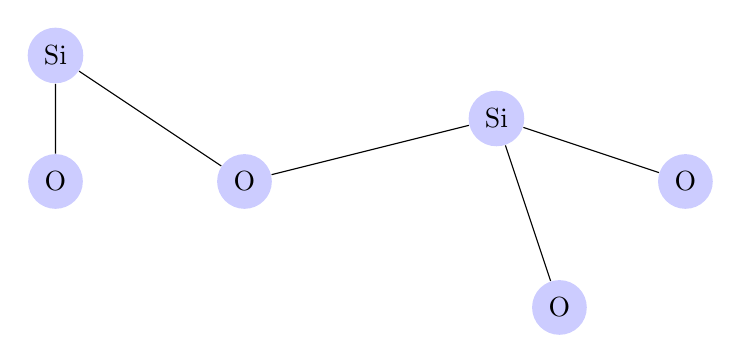
\begin{tikzpicture}
      [scale=.8,auto=left,every node/.style={circle,fill=blue!20}]
      \node (n6) at (1,10) {Si};
      \node (n4) at (4,8)  {O};
      \node (n5) at (8,9)  {Si};
      \node (n1) at (11,8) {O};
      \node (n2) at (9,6)  {O};
      \node (n7) at (1,8)  {O};
    
      \foreach \from/\to in {n6/n4,n4/n5,n5/n1,n2/n5,n6/n7}
        \draw (\from) -- (\to);
    
    \end{tikzpicture}
\caption{Basic graph representation, where nodes denote either silicon or oxygen atoms and edges denote bonds between atoms.}
\label{fig:basic_graph}
\end{figure}

As uniaxial stress is applied to the material, bonds can break and form, whereas atoms are conserved.  Thus, the vertex set remains constant, with size $|V|=n$ given by the total number of atoms in the system, whereas the edge set evolves in time.  We then define $E(t)$ to be the edge set at time step (snapshot) $t$, and $G(t) = (V,E(t))$ to be the graph at time step $t$.

There are significant benefits to having vertices whose identities do not change over the course of the simulation.  When predicting whether or not an atom ends up on the boundary of a fracture, it is convenient to able to describe that atom by the same graph element at $t=0$ as at the time of prediction.  A drawback of this representation, however, is the resulting graph size for the samples that we will study.  Training an ML algorithm on graph inputs with 70,000 vertices may place excessive demands on computational resources.

% Consider a sample of $n$ atoms.  Define an atom, whether silicon or oxygen, as a vertex $v_i$, where $0 \leq i \leq n-1$ and a set of such vertices is $\mathbf{\textbf{V}} = \{v_0,v_1,...v_{n-1}\}$. An edge, $e_i$ is defined as a chemical bond between two atoms. A set of such edges is $\mathbf{E} = \{e_0,e_1,...e_{n-1}\}$. As uni-axial stress is applied to the material, edges could break and form between any two vertices, where state 1 means an edge is broken and state 0 means an edge exists.
    %Therefore, a set of active edges, defined as $\mathbf{E_a}$, includes all the edges that have broke or formed at least once, meaning they have changed their state, either from 1 to 0 or from 0 to 1 at one point. Similarly, $\mathbf{V_a}$ is defined as a set of active atoms.
% As a result, the graph $\mathbf{\textbf{G}}$ is thus defined as a discrete set of vertices $\mathbf{V}$ connected by a set of edges $\mathbf{E}$. We can denote it as $\ \mathbf{G} = (\mathbf{V},\mathbf{E})$, where the size of the graph is $\ |\mathbf{V}| = n $.

    
\subsubsection{Reduced Graph Representation} 

An alternative graph representation is to consider only silicon atoms as nodes, and bonds through bridging oxygen atoms as edges.  Given the atomic content of SiO$_2$, this representation reduces the number of vertices approximately threefold, to 25,000 or less.  It also simplifies the encoding of Q$_n$ information, as a node with degree $n$ necessarily bonds to $n$ bridging oxygens, and thus forms a Q$_n$ unit.

Like the basic graph representation described previously, this reduced representation keeps the number of vertices constant.  On the other hand, it does not explicitly track bonds that are formed and broken at each time step: if a bond is broken in an Si--O--Si bridge, this representation will not distinguish between the case where the first bond, or the second bond, or both, are broken.  Similarly, the coordination number of an Si atom will not be given explicitly by node degree.  However, this information can, if needed, be encoded as feature information (see below).

\subsubsection{Additional Graph Formulations}

We will also explore additional means of representing the network.  One possibility may be in terms of ring structure.  Ebrahem et al.~\cite{ebrahem2018influence} have studied medium-range order in silica glasses, expressed by the sizes of rings of alternating Si and O atoms, which correspond to cycles in the two graph representations discussed above.  These ring size statistics appear to influence the tensile strength of SiO$_2$, with a flatter distribution of sizes accelerating the fracturing process, and a more sharply peaked distribution (larger number of medium-sized rings) delaying it.

It is possible that, by letting vertices represent rings with vertex labels describing ring size, we may obtain useful predictions of fracture locations. This approach would provide a very significant reduction of graph size.  It would have the limitation, however, that the vertex set would not remain constant from one time step to the next.  As bonds break and form, the composition of the rings change, and it may be challenging to interpret what a particular $t=0$ ring becomes at a later time.

% It is also shown that when the quench rate increases there was an increase in the number of large-sized rings and a decrease in the number of medium-sized rings. The change in the number of small-sized rings was minimal. Since there is larger void in large-sized ring, it can be stretched and deformed more than the medium-sized ring. However, a medium-sized ring can take more per unit stress while tensile is applied, so it has more strain energy \cite{mWilson_continuum_stress}.

% Typically in these silicate glasses there exists a structure where silicon (Si) is surrounded by four oxygen (O) atoms forming a tetrahedron seen in Figure 1. These tetrahedra share one common O atom if they are neighbors. A ring forms if a group of tetrahedra share common O atoms, and the size of these rings is computed based on how many Si atoms are in the ring. A large ring has 11 and 12 Si atoms, medium rings have 5 and 6, and small rings have 1 or 2. An atom is denoted as under-coordinated if the number of its constraints is lower than 4, and over-constrained, if greater than 4. \cite{pedone2015dynamics}
% \begin{figure}
%     \centering
%     \noindent
%     \includegraphics[width=12cm, height=6cm]{picture/tetra.JPG}
%     \caption{Example of a primitive sixfold ring (left), example of a primitive twelve-fold ring
% (right) \cite{ebrahem2018influence}}
%     \label{crack_Fig}
% \end{figure}

\subsection{Feature Description}
\label{subsec: Features}

% To use ML algorithms, we want to examine features of our system such as centrality, volume, and structure.

Given a graph representation, we may associate features with the nodes (as well as, in principle, the edges) of the graph.  Our ML algorithm can use these features to describe data points in the training set, learning a function that maps feature values to an output label.  The challenge is to identify features that are likely to have predictive value for the output label of interest, namely whether a node is on the boundary of a fracture.

%For instance, given $k$ features, a particular vertex $v_i$ may be described as a point $x_i\in\mathbb{R}^k$.  Predicting whether that vertex is on the boundary of a fracture at a subsequent time then corresponds to learning a function $y_i=f(x_1,\dots,x_n)$, where $y_i$ is the 

The work of previous CGU Math Clinic projects~\cite{valera2018machine,schwarzer2019learning} on graph-based ML for fracture prediction has suggested that different categories of features can be useful. Some of these are quantities that describe physical properties of an atom.  Others are local topological measures, that describe the network structure in the immediate proximity of a node. Finally, there are global topological measures, that describe ``centrality'' properties quantifying the importance of a node to network processes on the network such as communication or flow.

We propose a range of candidate features that are meaningful both for the basic and for the reduced graph representations.  For other formulations, such as in terms of ring structure, further study will be needed to determine appropriate quantities.  Furthermore, not all features that we initially propose will be significant for model predictions.  After running our ML algorithms based on these features, we will perform feature analysis to determine which characteristics of the system play an important role in the accuracy of predictions.

\subsubsection{Physical Features}
\label{subsubsec: Physical Features}

\begin{itemize}
%    \item \textbf{Atom type:} In the basic graph representation, vertices can denote both silicon and oxygen atoms.  In order to distinguish between them, a binary-valued feature may be assigned to a vertex that identifies which type of atom it is.  This feature would not be needed in the reduced graph representation, where vertices necessarily denote silicon atoms.
    
    \item \textbf{Cell volume:} A local density measure is given by the Voronoi diagram that partitions the system into polygonal cells surrounding each atom.  We define $v_i(t)$ to be the Voronoi cell volume of atom $i$ at time $t$.  These cell volumes can help our model understand which atoms are closely associated with fracture nucleation, by learning how and where volume increases.  When a fracture emerges, atoms on its boundary will have rapidly increasing cell volumes representing newly available space in the void.
    
    Note that while atoms on the boundary of a free surface can also have very large cell volumes, these volumes will already be large at $t=0$ and will typically not grow during the simulation.  A model that correctly learns the dynamics of cell volumes should therefore avoid mistaking the free surface for a fracture.

    \item \textbf{Atom displacement:} As fractures nucleate, atoms on its boundary may undergo more rapid displacement than do others.  Let $\mathbf{r}_i(t)$ be the vector representing the $(x,y,z)$ position of atom $i$ at time $t$. The physical displacement of an atom from one time step to the next, $\Delta \mathbf{r}(t)=\mathbf{r}_i(t)-\mathbf{r}_i(t-1)$, could help in predicting where and when fractures grow. 

    \item\textbf{Stress tensor:} The Cauchy stress tensor $\boldsymbol{\sigma}$ describes the local stress at each atom.  It may be the case that, prior to fracture growth, atoms that will ultimately form the fracture boundary undergo changes in values of their stress tensor components~\cite{elastic_fracture}. Note that, even in the absence of fracturing, considerable local fluctuations may occur in these values from one atom to the next.  Some form of spatial averaging may help in reducing these fluctuations.

    \item\textbf{Charge:} The emergence of fractures arises most directly from bond breaking.  The charge of an atom plays a crucial role in this.  As with the stress tensor components, we expect that atoms on a fracture boundary may, prior to fracture growth, exhibit characteristic changes in charge value.
%    We will take the charge of each atom in account to examine what effect each charge has in forming a fracture. The real values in our data represent the effects of quantum fluctuations from shifts of electron clouds. It is important to note that high charges indicate strong forces between atoms. Therefore, there is more activity. We want to investigate whether high charges are directly associated to active sets.
\end{itemize}

\subsubsection{Local Topological Features}

\begin{itemize}
    \item \textbf{Coordination number:} The coordination number of an atom is the number of neighboring atoms to which it is bonded.  Undercoordination and overcoordination could play a role in determing whether an atom will be on the boundary of a fracture.
    
    In our basic graph representation, the coordination number is equivalent to the degree of a vertex.  Even though it is implicit in the graph structure, however, there can be value in including it as an explicit feature for an ML algorithm to learn.
    
    In our reduced graph representation, the coordination number cannot be inferred from the graph at all, and must be included explicitly.
% We will use Degree Centrality Measures. These measures indicates how connected a vertex is by counting the direct links each vertex has to other vertices. Our network will be simplified to active bonds, therefore, the more links a vertex has to other vertices, the more connected that vertex is to active bonds. This will allow us to better understand where a fracture propagates from.

    \item\textbf{Number of bridging oxygens:} In a Q$_n$ unit, an Si atom is surrounded by $n$ bridging O atoms, each forming an Si--O--Si group.  The value of $n$ therefore supplies crucial network connectivity information. 
    
    In our reduced graph representation, the number of bridging oxygens is equivalent to the degree of a vertex.  Even though it is implicit in the graph structure (as with coordination number in the basic graph representation), ML algorithms may benefit from having it as an explicit feature.
    
    In our basic graph representation, this quantity would only be of direct use for those vertices that denote silicon atoms.  However, by setting it to a value of 0 for oxygen atoms, it could provide a means of distinguishing which type of atom a vertex represents: Si or O.

    \item\textbf{$k$th neighbor quantities:} A crucial assumption in our modeling approach is that structure beyond nearest-neighbor information can help in predicting fracture nucleation.  We therefore propose considering not only the number of bridging O atoms directly bonded to an Si atom, but also the number within a given number of bonds from an Si atom.
    
    In the reduced graph representation, a qualitatively similar quantity would be the following.  For an atom $i$ at time $t$, let $b^{(k)}_i(t)$ be the number of vertices whose path length to $i$ consists of at most $k$ edges. This defines a class of features for different values of $k$.  For $k=1$, $b^{(1)}_i(t)$ would simply be the vertex degree, i.e.,\ the number of bridging oxygens around $i$.  For increasing $k$, these features would consider local neighborhoods (around $i$) of increasing size.
    
\end{itemize}

\subsubsection{Global Topological Features}

% In network theory, centrality is used to quantify the importance of nodes to processes on the network, such as communication or flow.  Previous research on fracture networks has found that different forms of centrality can help predict properties related to fractures~\cite{santiago2016,valera2018machine}. An example could be a specific silicon atom that is at the center of where a fracture nucleates. Identifying the vertices with the highest centrality will allow us to predict fracture nucleation.

% More specifically, the vertex with the highest centrality degree would be surrounded by the most active bonds. Bonds that are not active do not necessarily contribute to the nucleation of a fracture \cite{valera2018machine}.
    
\begin{itemize}
    
    \item \textbf{Eigenvector centrality:} The influence of a specific node on a network is described not only by local properties of the node.  For instance, a node may have high degree but still not play a central role in processes on the network such as flow or communication.  Eigenvector centrality is one way of quantifying a node's global influence.
    
    Given an adjacency matrix $\mathbf{A}$ for a graph, where element $A_{ij}=1$ if an edge connects nodes $i$ and $j$ and $A_{ij}=0$ otherwise, the eigenvector centrality $e_i$ of node $i$ is the $i$th component of the leading eigenvector of $A$.  It satisfies
    \begin{equation}
    \lambda_{\max}(\mathbf{A}) e_i = \sum_{j=1}^n A_{ij}e_j,
    \end{equation}
    where $\lambda_{\max}(\mathbf{A})$ is the largest eigenvalue of $\mathbf{A}$.  The recursive nature of this equation reflects the intuition that an influential node is one that links to other influential nodes.  Previous research on fracture networks has found that eigenvector centrality can help describe a node's influence on certain kinds of fracture behavior~\cite{santiago2016,valera2018machine}, suggesting that it could be a relevant feature for predicting fracture growth.
    
%    Additionally, we want to use the local properties of the atoms as features. The local features are available from the molecular dynamics post processing data. This includes the size of a fracture and the speed of propagation. We aim to use eigenvector centrality measure which will lend a deeper understand as to what the connections a vertex with a high degree centrality has to the entire network. This is because eigenvector centrality measures the influence that a vertex has on an entire graph. Therefore, we can examine vertices that are associated with fractures and analyze what their effect is on the overall behavior of the glass.
    
%    Eigenvector Centrality Measures indicates how much influence a specific vertex has on the entire network. For example, consider a vertex that has a high degree centrality, but does not necessarily affect the network. Therefore, it must have a low eigenvector centrality and does not contribute to a fracture that significantly damages the network. For this reason, we want to consider which vertices have a high eigenvector centrality measure in connection with degree measures. Doing so will lead us to a deeper understanding of where fractures nucleate and what the propagation of  these fractures looks like.
    
    \item\textbf{Betweenness centrality:} A further global measure of node influence is the number of paths in the network that pass through that node.  This reflects the node's importance in communication across the network, which is relevant when the effects of uniaxial stress are distributed over the network.  Betweenness centrality counts the fraction of geodesic paths (paths with fewest possible edges) that include a given node.
    
    If $\pi_{uv}$ is the total number of geodesic paths connecting node $u$ to node $v$, and $\pi_{uv}(i)$ is the number of such paths that pass through node $i$, then the betweenness centrality of node $i$ is given by
    \begin{equation}
    \beta_i = \sum_{\substack{u,v = 1 \\ u\neq i\neq v }}^n \frac{\pi_{uv}(i)}{\pi_{uv}}.
    \end{equation}
    If the simulated sample had free boundary conditions in the direction of loading ($x$ direction), it is possible that relevant paths would only be those between a node $u$ along the left-hand boundary and a node $v$ along the right-hand boundary.  Since we are instead working with periodic boundary conditions in the $x$ directions, we will explore other possible ways of limiting the paths counted in the sum above.

\end{itemize}

\subsection{Extracting Ground Truth}


In this project, we will use a supervised learning technique. To train a supervised machine learning model, examples of input-output pairs are needed. Each of these pairs have the input and the corresponding desired output, which we call the ground truth.

In our model, the most straightforward ground truth is an indicator variable $\phi_i(t) \in\{0,1\}$, specifying whether or not atom $i$ is part of a fracture at time $t$.
%If $y_i=0$ is in state 0, it means it is not part of a fracture, and $y_i$ is in state 1, it means it is part of a fracture.
Given a system with $n$ atoms, $\boldsymbol{\phi}(t)$ is a binary vector of length $n$.  An important consideration, however, is that the simulation data described in Section~\ref{sec: Data} does not directly give ground truth information.  Instead, the ground truth must be extracted from other simulation output.

A fracture involves the creation of a void in the material. When stress is applied uniaxially, bonds break and form.  As a fracture nucleates, some atoms are on the boundary of the emerging void, while others are compressed into denser regions.  Consequently, we define the ground truth using a local density measure closely related to the first of the physical features described above.  Consider the Voronoi cell volume $v_i(t)$ of atom $i$ at time $t$.  When this volume exceeds a certain threshold, we consider atom $i$ to be part of a fracture event.  Figure~\ref{fig:crack_vol} highlights in red the atoms that would be identified in this way with a fixed threshold value, on a snapshot from a dry simulation with fully periodic boundary conditions.

    \begin{figure}
    \centering
    \noindent
    \includegraphics[width=8cm, height=6cm]{picture/volcolor.PNG}
    \caption{Atoms in red are those with Voronoi cell volume $v_i>42$.  Dark areas are voids that represent fractures.}
    \label{fig:crack_vol}
    \end{figure}
    
In order to establish the ground truth, we will set the threshold value for a given time $t$ to be equal to three standard deviations above the mean Voronoi cell volume at that time.  Thus, we test whether the standardized cell volume
    \begin{equation}
    \hat{v}_i(t) = \frac{v_i(t) - \mu_v(t)}{\sigma_v(t)} > 3,
    \end{equation}
where $\mu_v(t)$ is the mean and $\sigma_v(t)$ is the standard deviation of $v_i(t)$ over all $i\in\{1,\dots,n\}$.  Note that in the postprocessed nucleation data supplied with the simulations, this is equivalent to testing whether the quantity in the field {\tt nuc\_v} exceeds 1.

Because of the effects of free surfaces discussed in Section~\ref{subsubsec: Physical Features} above, $v_i(t)$ must be modified to disregard cell volumes that are large because they are on the boundary of a surface rather than a fracture.  Since these cell volumes do not significantly change over time, we define a new quantity that subtracts out the $t=0$ value, $v'_i(t) = v_i(t)-v_i(0)$, and instead test whether
\begin{equation}
    \label{eqn: cell volume}
    \hat{v}'_i(t) = \frac{v'_i(t) - \mu_{v'}(t)}{\sigma_{v'}(t)} > 3.
\end{equation}
The ground truth can then be defined:
\begin{equation}
    \label{eqn: ground truth}
    \phi_i(t) = \begin{cases}
      0 & \text{if }\hat{v}'_i(t) \le 3 \\
      1 & \text{if }\hat{v}'_i(t) > 3 \\
    \end{cases} 
\end{equation}

We will apply two further corrections to $\phi_i(t)$, to limit the case of false negatives (where atoms on the boundary are identified as $\phi_i(t)=0$) as well as false positives (where atoms not on the boundary of a fracture are identified as $\phi_i(t)=1$).

The false negative case occurs when an atom is at the boundary of a fracture, but is surrounded by a sufficient number of other nearby atoms that its Voronoi cell volume does not extend out into the void.  To account for this, we will consider a small neighborhood around each positively identified atom $i$.  Any other atom whose path length to $i$ consists of fewer than a small number of edges (such as 2 or 3) will be considered to be on the boundary as well.

The false positive case occurs early in the simulation, prior to nucleation, when the standard deviation $\sigma_{v'}(t)$ is very small, and atoms can be identified as positive purely due to spatial fluctuations in density.  To reduce this problem, we use the fact that an atom on the boundary of a fracture at time $t$ is expected to remain on the boundary of a fracture for the remainder of the simulation.  If an atom is positively identified, we will test whether it remains positively identified for the majority of the remaining simulation times.  If not, it will not be considered to be on the boundary.

Finally, we propose an alternative to extracting information from simulations on whether an atom is at a fracture boundary, and then training our algorithms using this ground truth.  Instead, we can simply adopt the cell volumes as ground truth, and train our algorithms to predict this.  Our predictions may then be postprocessed using Equations~(\ref{eqn: cell volume}) and (\ref{eqn: ground truth}) to determine which atoms are at fracture boundaries.  This could have the advantage of providing a more objective prediction, but involves solving a regression problem rather than merely a classification problem.

\subsection{Machine Learning Methods}

The objective of this project is to produce a surrogate model of the molecular dynamic simulations using supervised machine learning techniques. We propose to address our two goals listed in Section~\ref{sec: Goals} with two methods, respectively. First, we will use ensemble methods such as random forest to predict nucleation at a fixed future time step, given feature information at $t=0$.
%We will use an ensemble of random forest to predict nucleation based on local structures.
% Second, predict the Vonoroi volume of an atom, and use the prediction to interpret whether or not an atom is part of the fracture. Therefore this section of the methods will address our proposed ML architecture from start to finish.
Second, we will use a recurrent neural network (RNN) with the long-short term memory (LSTM) mechanism, to learn the dynamic process of fracture propagation. % LSTM has the benefit of being a flexible model, where we can control how much memory we would like the model to contain when making predictions.

\subsubsection{Random Forest for Predicting Fracture Nucleation}
%\item \textbf{Method for Classifying whether or not a vertex is part of a fracture in the nucleation setting}

%Random forest. Boosting, bagging. 
For the purpose of determining whether or not a node is associated with a fracture, we will implement ensemble-based ML methods. The goal of ensemble methods is to combine predictions made by several features into one single learned estimator. With our feature selection being possibly quite large, we will find ensemble methods the best option to predict fracture labels. 

Core ensemble methods include bagging and boosting. A ``bagged'' random forest method is generated by creating a tree from features randomly drawn with replacement. 
% Since our representation is graph-like these trees make sense logically. 

Our bagging algorithm will work as follows:

\begin{enumerate}
\item Take training set $T$ with $N$ features, with $L$ models.
\item For model $L _{1}$ let the number of input points $n_{1}$ $<$ $N$ for each $L_{n}$.
\item For model $L_{n}$, create a training set by choosing $d_{l}$ features from T with replacement and train the model.
\end{enumerate}

Adaboost, on the other hand, is a boosting method that learns from previous mistakes made during training. By doing so, the model can increase the weights of incorrectly predicted points from the training data.

Our boosting algorithm will work as follows:

\begin{enumerate}
    \item Initialize weights of the features.
    \item Train a decision tree.
    \item Find the error weighed rate and calculate the tree's weight in the overall ensemble.
    \item For every feature wrongly predicted, update the weight.
    \item Repeat until complete. 
\end{enumerate}

%\item \textbf{Method for Predicting the Voronoi Cell Volume Dynamically}

\subsubsection{Fracture Propagation}
%RNN, 
Due to the dynamical nature of our graph changing over each time step, we will be implementing an RNN to predict the ground truth at each time step. An illustration of the basic RNN architecture is shown in Figure~\ref{fig:rnn}.  The main idea behind an RNN is that it trains on an entire time series, learning the dynamics of a process which it stores using a ``memory'' of internal states.  The LSTM mechanism is a refinement of this memory, allowing the neural network to give added weight to information learned in more recent time steps.

\begin{figure}
    \centering
    \noindent
\includegraphics[width=12cm , height = 5cm]{picture/rnn.PNG}
    \caption{Representation of a Recurrent Neural Network}
    \label{fig:rnn}
\end{figure}


The training input to our RNN will be a time series of graphs based on simulation data, where nodes will be labeled with the full set of feature values described in Section~\ref{subsec: Features}.  For every time $t$, the RNN outputs feature and ground truth values for time $t+1$.  These are compared with simulation results, from which a loss function is calculated and the internal neural network weights are updated.

Once the RNN is trained and its weights are set, it is used for prediction.  The input at this point is simply the $t=0$ feature values, but the output is a time series of graphs, giving the full predicted evolution of features and ground truth.

Note that certain of our features, such as atom displacement, are undefined at $t=0$ and thus are meaningful only as part of the training process.  Others, however, are well-defined at any individual time step.

% Voronoi cell volume for all the atoms at time step $t$, which is a vector of length $n$.

% After we have obtained a time series of predicted $v_i$, we compare the prediction with the threshold, which is 3 standard deviations from the mean, to determine whether a certain atom is part of a fracture or not. Similar with what is defined before:
%    \[
%     \hat{y_i} = \begin{cases}
%       0 & \text{if }(nuc_v)_i \le 1\\
%       1 & \text{if }(nuc_v)_i > 1\\
%     \end{cases} 
%     \]  

\subsubsection{Algorithmic Architecture}
% \item \textbf{Machine Learning from start to finish}

The proposed architecture is as follows:

\bigskip

\begin{center}
\tikzstyle{decision} = [diamond, draw, fill=blue!20, 
    text width=4.5em, text badly centered, node distance=3cm, inner sep=0pt]
\tikzstyle{block} = [rectangle, draw, fill=blue!20, 
    text width=5em, text centered, rounded corners, minimum height=4em]
\tikzstyle{line} = [draw, -latex']
\tikzstyle{cloud} = [draw, ellipse,fill=red!20, node distance=3cm,
    minimum height=2em]
    
\begin{tikzpicture}[node distance = 2cm, auto]
    % Place nodes
    \node [block] (init) {MD Simulation Data};
    \node [block, below of=init] (features) {Extracted Features};
    \node [block, below of=features] (training) {Training Set};
    \node [block, left of=training, node distance=3cm] (test) {Test Set};
    \node [block, right of=training, node distance=3cm] (validate) {Validation Set};
    \node [decision, below of = training] (RF) {Random Forest};
    \node [decision, below  of = test] (rnn) {LSTM};
    \node [cloud, below of = RF] (out) {Surrogate Model};
    %\node [cloud, below of= RF, node distance=3cm] (pof) {RF Output};
    %\node [cloud, below of= rnn, node distance=3cm] (rnnout) {RNN Output};

    % Draw edges
    \path [line] (init) -- (features);
    \path [line] (features) -- (validate);
    \path [line] (features) -- (training);
    \path [line] (features) -- (test);
    \path [line] (training) -- (RF);
    \path [line] (training) -- (rnn);
    \path [line] (rnn) -- (out);
    \path [line] (RF) -- (out);
    \path [line] (validate) |- node [near end] {} (out);
\end{tikzpicture}
\end{center}

\begin{enumerate}
    \item Analyze and determine features from the MD data.
    \item Extract the features and prepare data for training.
    \item Split the dataset into three sets: training, validation, and test
    \item
    \begin{enumerate}
        \item Train the training set using RF to predict which atoms are part of a fracture.
        \item Train the data using LSTM to predict fracture evolution.
    \end{enumerate}
    \item Validate surrogate model using validation set.
    \item Feature analysis. Fine tune features which are deemed most important. 
    \item Finalize surrogate model on test set. 
\end{enumerate}

\section{Milestones}
\label{sec: Milestones}
\begin{enumerate}

    \item \emph{Find an appropriate graph representation: }

    \begin{itemize}
    %\emph{Predicting Fracture Nucleation Events} 
        Option 1: We define each atom, either a Si or Oxygen, as a node. Each node has features associated with it, such as position (defined by coordinates), charge, stress tensor, and bond information. An edge is the bond relationship between two nodes. There are no special features of the edges. Any fracture nucleation event originates from bonds breaking, which could happen between any pair of nodes, but especially those between Si and Oxygen atoms.
        \\
        Option 2: we define each node as a molecule, meaning one Si atom bonded with four oxygen. While stress is applied to the glass, bonds between atoms and molecules break. As atoms are pulled away from each other, the size of a node changes as well.
        
        \item \emph{Define fracture within our graph} : 
        \\Based on the basic graph defined previously, we want to define a fracture. To do so, we consider the following approaches:
        \begin{itemize}
            \item Radial distribution
            \item KNN
            \item Simple distance
        \end{itemize}
    \end{itemize}

    \item \emph{Predicting Fracture Propagation} 


            Based on the given data, we have snapshots in time of the dynamic process. For each  atom, each snapshot contains coordinates for position, charge, stress tensor, and bond information, such as connectivity. We will define our features using these four data.
        \begin{itemize}
            \item Position using distance matrix
            \item Charge
            \item Stress tensor
            \item Bond information. We utilize the local structure of the glass, where we have $Q_3$, $Q_4$, and $Q_5$. We will do so by using adjacency matrices.
        \end{itemize}

    \item \emph{Identifying Regions of Fractures} 
        \begin{itemize}
            \item To label and predict the nucleation of fractures, we must first identify the atoms that are in the process zone of a fracture. 
            \item Computing the convex hull of a graph of nodes is one way to represent the process zone occupied by the nodes.
        \end{itemize}
\end{enumerate}












\section{Deliverables}
\label{sec: Deliverables}
\begin{enumerate}
\item Graph representation implemented in Python. 
\item Midyear presentation.
\item Midyear report. 
\item Machine Learning Model Produced
\item Journal article on our graph-theortic ML approaches.
\item Final presentation
\item Final Report
\item Site visit and presentation at Sandia National Laboratory.  

\end{enumerate}


\section{Schedule}
\label{sec: Schedule}
\begin{tabular}{ l|l } 
 \hline
 Date & Description  \\
 \hline
 November 20, 2019 & Midyear Presentation at CGU   \\ 
 December 20, 2019 & Midyear Report \\ 
 May 5, 2020 & Final Presentation at CGU \\ 
 May 12, 2020 & Completion of Project \\ 
 TBD & Site Visit and Presentation at Sandia National Laboratory  \\ 
\end{tabular}\\

%%% Appendices.

%%% For your Statement of Work, you probably won't have any
%%% appendices, but you could include some if you really needed to.

%%% The appendices are delineated with the \appendix command.
%%% Individual appendices are begun with the standard \chapter or
%%% \section commands.  In our example, we'll \include them just as we
%%% did other chapters.

%%% Even in a relatively short document such as your statement of
%%% work, you might need to have appendices.  If so, uncomment
%%% the \appendix command and add them below (remember, the
%%% top-level structural command in this format is section).

% \appendix


%%% Bibliography.

%%% BibTeX is the tool to use for citations and layout of your
%%% bibliography.  Instead of having to type ``[5]'' or ``(Jones,
%%% 1968)'' (and keep track of which citation is which and renumber
%%% them as you add more references to your bibilography), you use
%%% special commands that allow BibTeX and LaTeX to automatically put
%%% the correct information in the right place.

%%% Section 5.6 in _The Mathematics Clinic in Brief: A Handbook_,
%%% talks about using BibTeX to format your bibliography and
%%% citations.

%%% Depending on your field, it may or may not be appropriate to list
%%% references for which you haven't included specific citations.  If
%%% your field sanctions such practices, or if you just want to get an
%%% idea of what you have in your bibliography file, you can include
%%% everything with the \nocite{*} command.          

%%% The appearance of your bibliography and citations in your text are
%%% defined by a combination of any bibliography-related LaTeX
%%% packages (such as natbib, harvard, or chicago) and the particular
%%% bibliography style file that you load with the \bibliographystyle
%%% command.  Bibliography-style files end in .bst; you can find them
%%% by searching your file system using whatever tools you have for
%%% doing searches.  (On most modern Unices, ``locate .bst'' will give
%%% you an idea of what's available.)

%%%%\bibliographystyle{IEEEtran}

%%% The particular bibliography data file or files that you want to
%%% use are specified with the \bibliography file.  Multiple files are
%%% separated by commas.

%%% You might want to use multiple bibliography (or ``bib'') files if
%%% you had a master bib file containing references you use again and
%%% again, and another containing only records for references for a
%%% particular project.

%%% Many people create a single, large bib file that they use for
%%% everything they write.  That approach requires you to \cite every
%%% reference that you want to use in your document -- using
%%% \nocite{*} with a huge bibliography database will give you a large
`%%% bibliography containing many references you haven't consulted for
%%% your particular document!
\bibliographystyle{IEEEtran}
\small
%\nocite{*}
\bibliography{Bibliography}


%%% Glossary or Index.

%%% Having a glossary or index in a statement of work is overkill.
%%% Just define your terms in the text and you'll be fine.

\end{document}


